This chapter discusses the information theoretical analysis of the dataset. The source code developed for the analysis has been implemented in the Python programming language. The actual implementation will be discussed in-depth in chapter~\ref{implementation}. 

The dataset contains the source-reconstructed data from four EEG channels. The datapoint within the dataset encompass 13 subjects. The source-reconstructed data from the abstractness and concreteness eperiment is given from 3 different regions. 

One region represents the cortical area which is active during both the abstractness and concreteness experiments. For this region, the data from both experiments are given. Another region represents the cortical area which is only active during the abstractness experiment and the final region represents the cortical area which is only active during the concreteness experiment. Finally, resting state data was available for all 3 regions.

First, this chapter will discuss the procedure for finding the amount of bins that will be used throughout the analysis. In order to be able to utilise the binning method for entropy estimation, the correct number of bins needs to be computed.

Afterwards, the main analysis is discussed. The common region which were active during both the abstractness and concreteness experiments are the main focus. Secondly, the analysis is adapted in order to analyse the different subjects  independently. Finally, an analysis was made for a comparison between the active regions and the resting state counter parts.

\section{Calculating Bin Sizes}

Section~\ref{binning} discussed the discretization of continuous data. There are multiple methods to calculate the optimal number of bins. The number of bins can be calculated empirically. This can be seen in figure~\ref{bins}. The entropy is calculated for a number of different bin sizes. Using this method, the entropy seems to converge for the bin sizes. The convergence starts from a bin size of about 100. This gives an indication for the optimal bin size.

\begin{figure}[!htb]
\caption{Entropy comparison between bin sizes}
\label{bins}
    \centering
    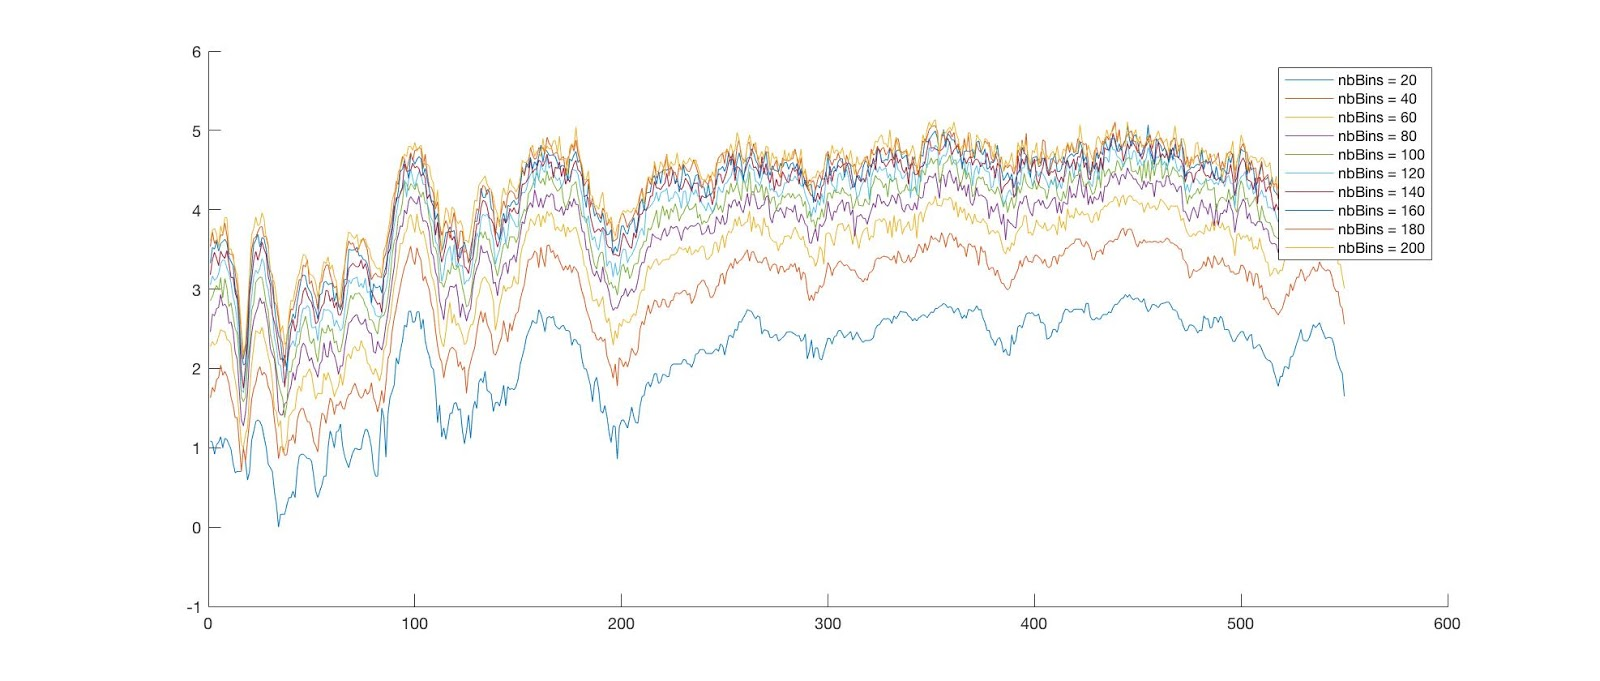
\includegraphics[width=1.2\textwidth]{fig/bins}
\end{figure}

There is also equation~\ref{binequation}. Using this equation, the optimal bin size is calculated to be 90. Both the equation and empirical method find approximately the same result. For the analysis, a bin size of 90 has been chosen. 

\section{Comparing the Common Region}\label{analysis1}

As explained before, the common region which were active during both the abstractness and concreteness experiments are the main focus. The main strength of an information theoretical approach is the measurement of mutual information. Mutual information can measure both linear and non-linear relationships. 

From the activity, we could see that some cortical areas are active during both the abstractness and concreteness experiments. Mutual information can tell us what kind of relationship there is between the abstractness and concreteness. There are several different possibilities. One theory is that the common region represents the semantic processing that is common between the abstractness and concreteness experiments.

Figure~\ref{all-channel-1} shows the results of the analysis. $Abs$, $Con$ and $Rest$ represents the information entropy through time. $Abs$ is the information entropy from the abstractness experiment. $Con$ is the information from the concreteness experiment. 

$Abs$ and $Con$ have about the same information entropy throughout time. This corresponds to the fact that this region is active and doing semantic processing. $Rest$ is the information entropy during resting state. 

\begin{figure}[!htb]
\caption{Experiment}
\label{all-channel-1}
    \centering
    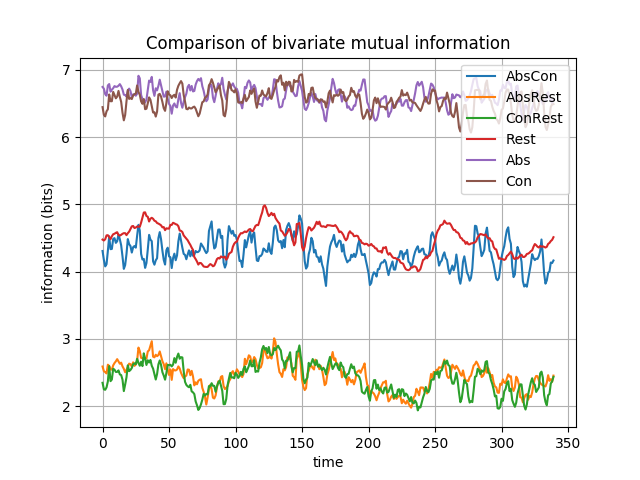
\includegraphics[width=\textwidth]{fig/all-channel-1}
\end{figure}

$AbsRest$ and $ConRest$ represent the mutual information between, respectively, abstractness and rest, and, concreteness and rest. The mutual information is much lower than the entropy from the resting state. This indicates that whatever is happening during resting state is very different from the activity during semantic processing. This is a small, but very important observation.

$AbsCon$ represents the mutual information between the abstractness experiment and the concreteness experiment. One observation is that $AbsCon$ is on an equal footing with the information entropy during the resting state. This can, wrongfully, lead to the conclusion that the only equal information between abstractness and concreteness is the activity that occurs during the resting state.

However, considering that $AbsRest$ and $ConRest$ are much lower, this conclusion cannot be made. This analysis finds that there is some mutual information between abstractness, concreteness and resting state. There is also some mutual information between the abstractness and concreteness, which is not completely caused by the resting state activity. 

Figure~\ref{venn} roughly visualizes these relationships information. There is some common information (rounded to 1 bits) between all 3 datasets. There is also some information that is unique to each of the datasets. Abstractness and concreteness share some information, which is unrelated to the resting state. This venn diagram helps visualize some results, but is very deceptive for visualizing multivariate mutual information.

There are some conclusions to be made from this. First of all, some of the semantic processing of abstractness and concreteness in the same cortical area is shared. However, it seems that the same cortical area does not compute exactly the same features during semantic processing of abstract and concrete words. 

\begin{figure}[!htb]
\caption{Venn Diagram for Information in Common Region \cite{venn}.}
\label{venn}
    \centering
    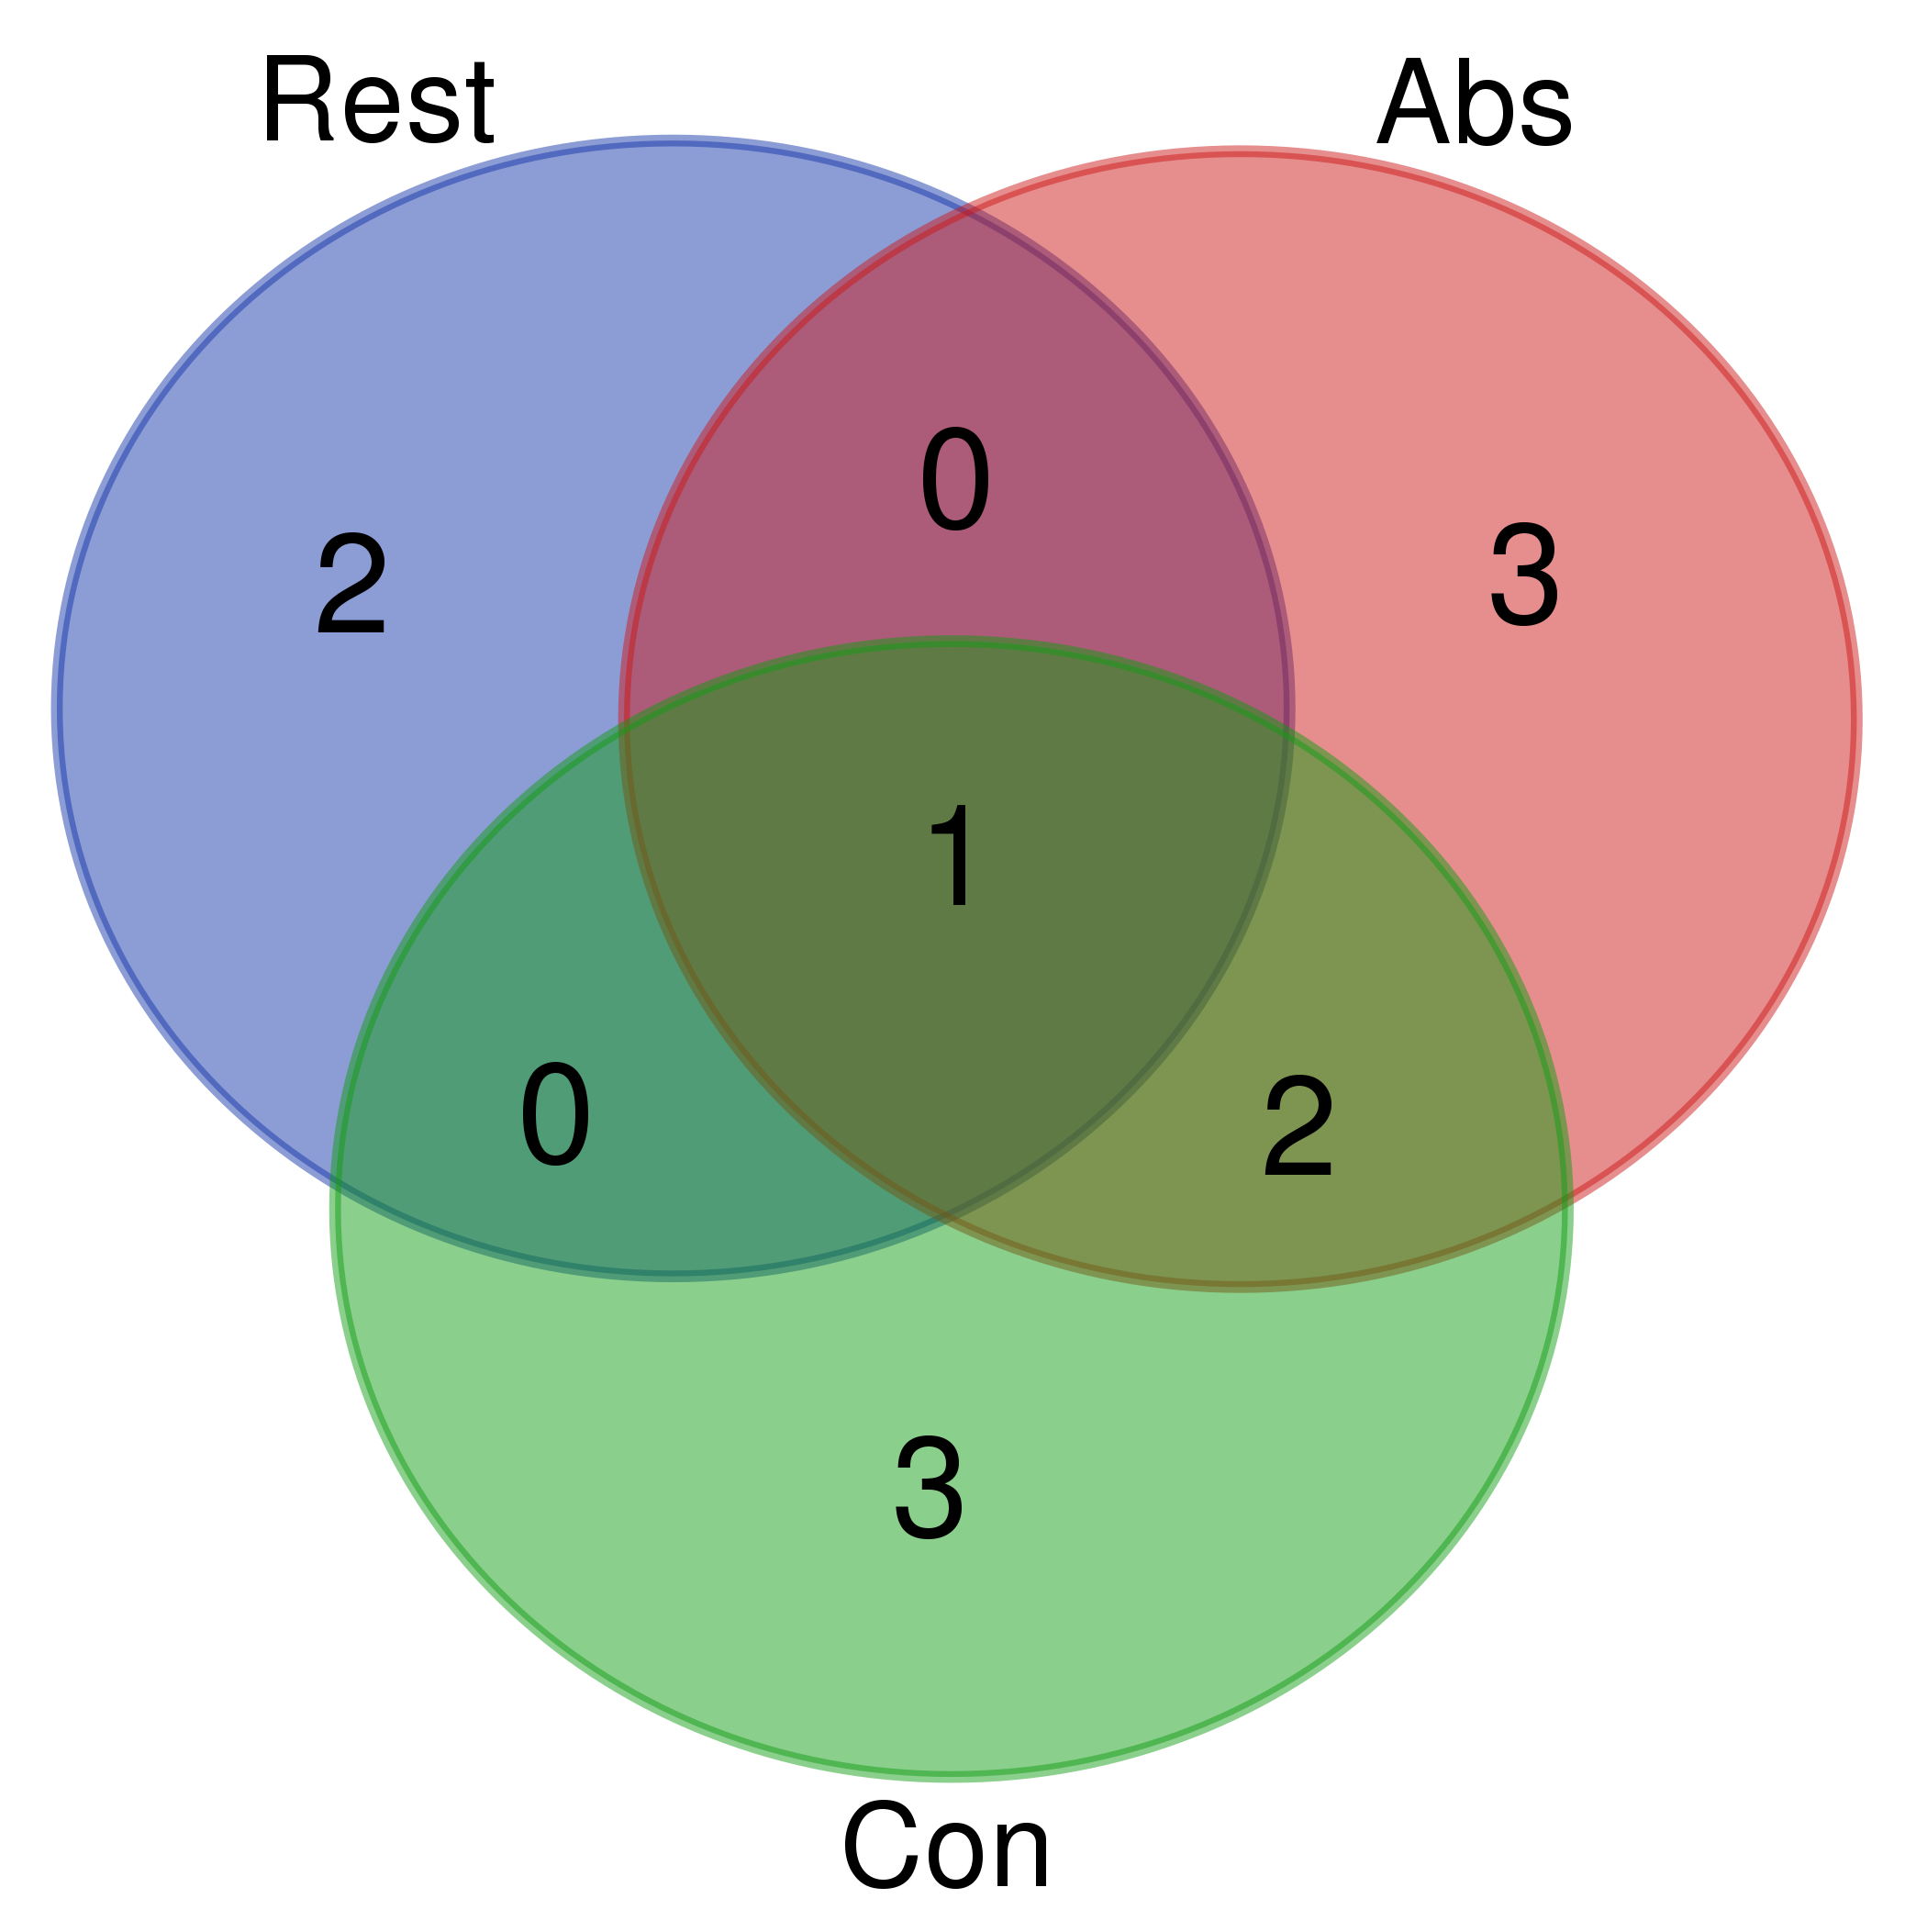
\includegraphics[width=0.8\textwidth]{fig/venn}
\end{figure}

Figure~\ref{comp-1} shows this relation expressed as percentages. About 60\% to 70\% of the activity is shared between the semantic processing of abstract and concrete words. This leaves 40\% to 30\% of the activity that is unique for the semantic processing of abstract words and for the semantic processing of concrete words.

\begin{figure}[!htb]
\caption{Comparison}
\label{comp-1}
    \centering
    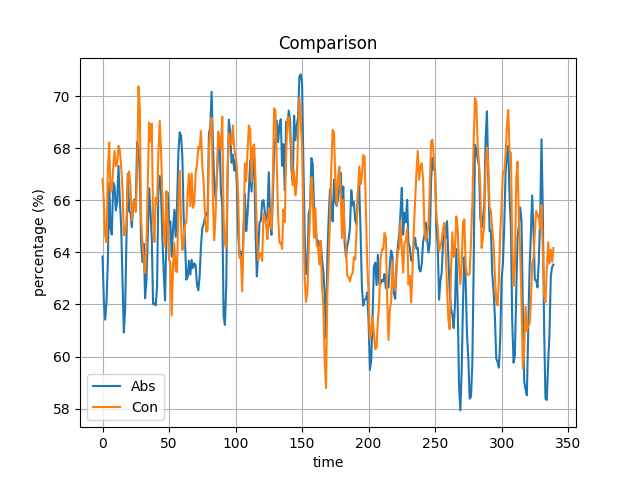
\includegraphics[width=\textwidth]{fig/comp-1}
\end{figure}

\section{Comparing the Common Region: Multivariate}\label{analysis2}

So far, bivariate mutual information has been utilised. However, there is also the multivariate mutual information. This can be used to calculate the mutual information between the abstractness, concreteness and resting state. 

Looking at figure~\ref{venn}, you would expect the multivariate mutual information to be 1 bit. However, the actual result is -1 bit, as seen in figure~\ref{mul-all-channel-1}. At first, this seems very strange. Having a negative amount of information is very counter-intuitive.

\begin{figure}[!htb]
\caption{Multivariate Experiment}
\label{mul-all-channel-1}
    \centering
    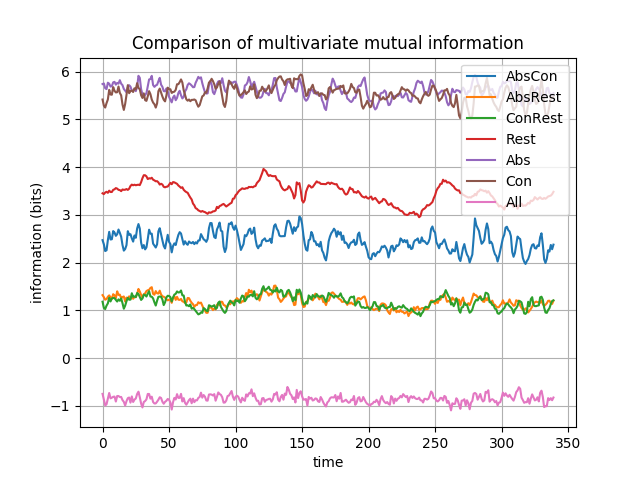
\includegraphics[width=\textwidth]{fig/mul-all-channel-1}
\end{figure}

Looking at the equation that is used for the multivariate mutual information, we get:

\begin{equation}
I(Abs, Con, Rest) = I(Abs, Con) - I(Abs, Con | Rest)
\end{equation}

Looking at figure~\ref{mul-all-channel-1}, we can see that $I(Abs, Con)$ has a value between 2 and 3 bits of information. However, $I(Abs, Con | Rest)$ is a bit more difficult. This can also be written as a sum of entropies:

\begin{equation}
I(Abs, Con | Rest) = H(Abs,Rest)+H(Con,Rest)-H(Abs, Con, Rest)-H(Rest)
\end{equation}

The deceptive point is that the joint entropy $H(Abs, Con, Rest)$ isn't as large as the venn diagram makes it look. The result is that $I(Abs, Con | Rest) > I(Abs, Con)$, which causes a negative multivariate mutual information. 

Negative multivariate mutual information indicates a synergy. Figure~\ref{common} shows a graphical model detailing this. $Z$ and $Y$ represent $Abs$ and $Con$, while $X$ represents $Rest$. $Rest$ causes a stronger dependency between $Abs$ and $Con$, than without $Rest$. This shows that multivariate mutual information is quite difficult to interpret.

\begin{figure}[H]
\caption{Multivariate Mutual Information Synergy}
\label{common}
    \centering
    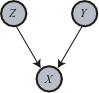
\includegraphics[]{fig/common}
\end{figure}
    

\section{Per Subject Comparison}

An per-subject analysis has also been performed. With a per-subject analysis, we can see whether results would vary between different subjects and whether there are different conclusions to be made.

Figure~\ref{all-trials} shows the analysis from section~\ref{analysis1} executed on a single subject. The figure looks very similar to figure~{all-channel-1}. This reaffirms the conclusion on a per-subject basis.

\begin{figure}[!htb]
\caption{Comparison for Subject 1}
\label{all-trials}
    \centering
    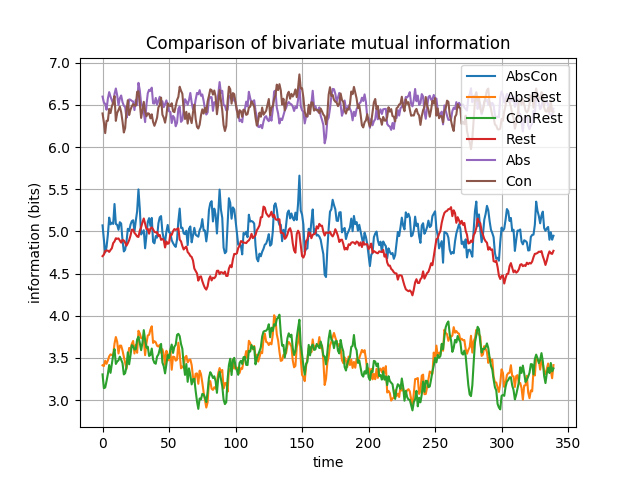
\includegraphics[width=\textwidth]{fig/subject1_alltrials_all-channel-1}
\end{figure}

\subsection{Effect of Trials Used}

Another interesting avenue to pursue was analysing the effect of the amount of trials used within information theoretical equations. In other words, how much data do we need in order to get decent results. We expected that information theory would still deliver good results, even with relatively few data.

Several additional analyses were performed. Each analysis used a different amount of trials. The complete dataset contains 3404 datapoints, with an average of 262 datapoints per subject (per timepoint). With binning being done with 90 bins, this means that there are about 3 datapoints in each bin. 

In order to see the effect of the amount of datapoints that are used, the information theoretical analysis was performed with 10, 40, 80 and 100 datapoints. 

Figure~\ref{10-trials} shows the result from only using 10 datapoints. With 90 bins, most bins are completely empty. Due to this, the computed information entropy is very inaccurate. 

\begin{figure}[!htb]
\caption{Comparison for Subject 1 - 10 datapoints}
\label{10-trials}
    \centering
    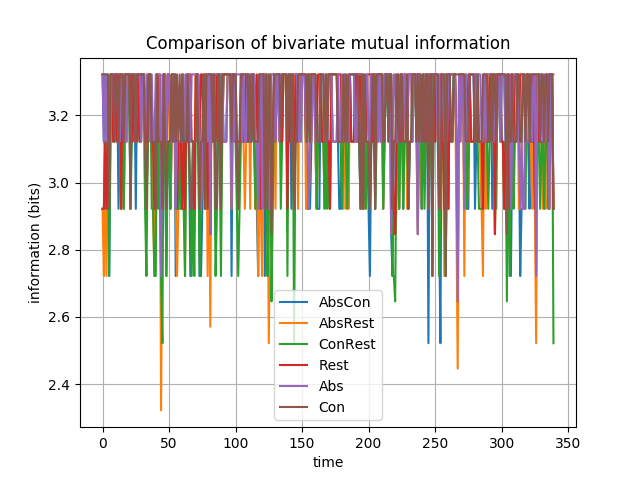
\includegraphics[width=\textwidth]{fig/subject1_10trials_all-channel-1}
\end{figure}

Figure~\ref{40-trials} shows the result from only using 40 datapoints. In this case, the result starts becoming more accurate.

\begin{figure}[!htb]
\caption{Comparison for Subject 1 - 40 datapoints}
\label{40-trials}
    \centering
    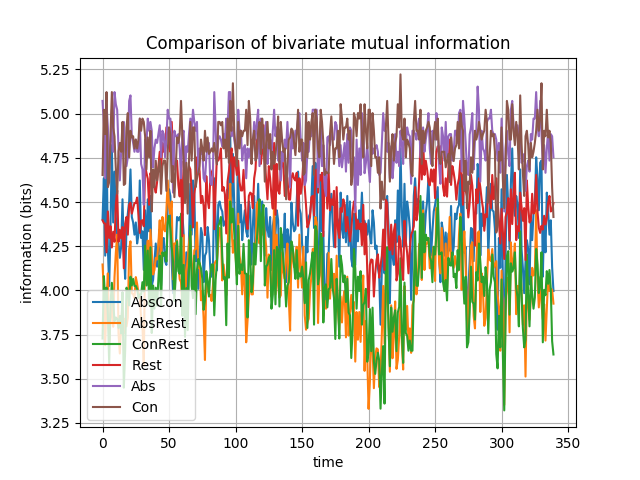
\includegraphics[width=\textwidth]{fig/subject1_40trials_all-channel-1}
\end{figure}

Figure~\ref{80-trials} shows the result from using 80 datapoints. With 80 datapoints, nearly every bin should be filled. From this point, the resolution starts becoming much more accurate. 

\begin{figure}[!htb]
\caption{Comparison for Subject 1 - 80 datapoints}
\label{80-trials}
    \centering
    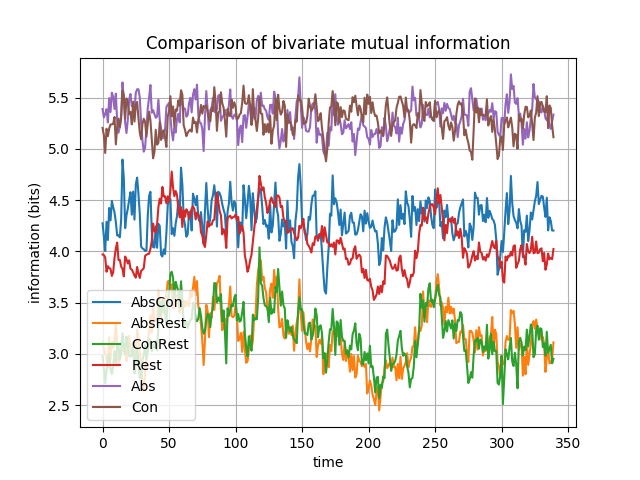
\includegraphics[width=\textwidth]{fig/subject1_80trials_all-channel-1}
\end{figure}

Figure~\ref{100-trials} shows the result from using 100 datapoints. The resolution increases yet again. However, the new details that are visible in the graph do not cause more conclusions or results to be drawn. 

This analysis shows that, if not enough data is available, information theoretical equations cannot reliably be used. For the 10 and 40 datapoint analyses, this is clearly shown. However, the 80 and 100 datapoint analyses show that even with relatively few datapoints, relative to the amount of bins used, the resolution is already quite clear.

\begin{figure}[!htb]
\caption{Comparison for Subject 1 - 100 datapoints}
\label{100-trials}
    \centering
    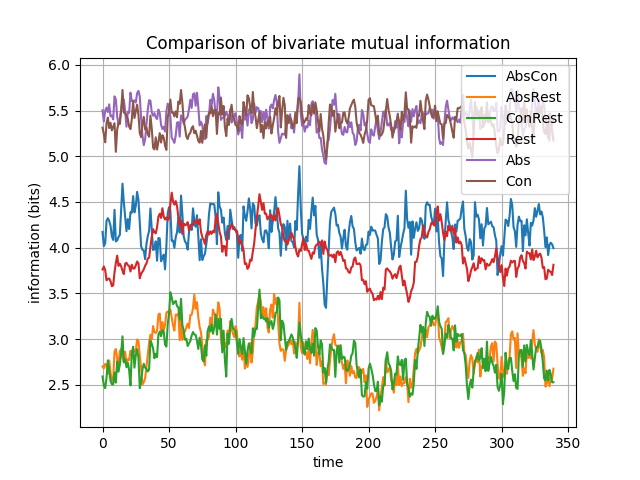
\includegraphics[width=\textwidth]{fig/subject1_100trials_all-channel-1}
\end{figure}

